\documentclass[11pt,a4paper,titlepage]{article}
\usepackage{graphicx}
\usepackage[margin=1in]{geometry}
%\usepackage{titling}
\usepackage{booktabs}
\usepackage[hidelinks]{hyperref}
\usepackage{float}


\usepackage{epstopdf}

\DeclareGraphicsExtensions{.png}
\DeclareGraphicsExtensions{.jpg}
%\DeclareGraphicsExtensions{.eps}

\begin{document}
\begin{titlepage}
	\begin{center}
		
		\begin{figure}[t]
			\centering
			
\includegraphics[width=350px]{UP_Logo.png}
		\end{figure}		
	
	
	\begin{flushright} 
		
		\textbf{\LARGE COS 301 Main Project}
		\newline \newline \newline
		\textbf{\LARGE Requirements and Design Specifications}
		\newline \newline \newline
 		\textbf{\LARGE ThinkTech}
		\newline \newline \newline
	\end{flushright}
		
		\vspace{1 cm}
		
		\LARGE{\textbf{Group Members: }}
		
		%\begin{minipage}{0.4\textwidth}

		\begin{flushright} \large
			Lelethu Zazaza 13028023\newline
			Goodness Adegbenro 13046412\newline
		\end{flushright}
		%\end{minipage}
		
	
		
		\textbf{Git repository link:\\}
		 \url{ https://github.com/COS301-ThinkTech}
		
		\vfill
		
		{\LARGE Version 0.1}
		\\
		{\large \today}		
		
		
	\end{center}
\end{titlepage}


\newpage
\tableofcontents


\pagebreak

\section{Background, Vision and Scope}
\subsection{Project background}
Without the correct or adeqaute number of resources, learning a new concept may turn out to be a daunting task. This is especially true for students who are studying a Computer Science course yet are not equipped with a practical or theoretical programming background. The motivation behind this project is to develop a tool that is intended to bridge the  gap between inexperience and practical application. The tool will provide the means to simulate program logic through flowcharts in a practical setting. 

\subsection{Project vision}

The aim of this project is to develop a flowchart and planning simulation tool that is simple and intuitive to use. Firstly, this will be accomplished by enhancing the visual nature of the application by making tools in certain contexts more prominent. Additionally, the application should provide informative and clear feedback to the user during the flowchart development phase. It is important that the look-and-feel of the application is uncluttered and uncomplicated so that the user feels at ease to experiment with the tools thereby enhancing the learning experience.

\subsection{Project scope}

The application is compromised of 2 units: flowchart development and flowchart simulation. An explanation of each unit will follow below.

\begin{itemize}
\item Flowchart development

The user is presented with a canvas upon which he can drop flowchart components to create a  complete flowchart.
The application will perform error checking on the constructed flowchart, so that (for example) multiple entry points into a program or certain flowchart components are not allowed. The applicatiom should also warn the user of instances of infinite loops or other  logical error possibilities. 

\item Flowchart simulation

The user should be able to run an error-free flowchart from start to finish. The system should allow for one-click execution of the entire program, as well as step-by-step execution. At all stages during execution, the currently executing component should be
highlighted, as well as the connection path being followed. The program's execution should
be very visually apparent and appealing. The output of the flowchart's execution should also
be apparent. 
\end{itemize}

The following components are specifically excluded from the scope of the project:

\begin{itemize}
\item No executable program code generation will be required for this project.
\item No complex design elements (such as user-defined component assemblies) are required.
Only the basic components of standard flowcharts are necessary.\\

\end{itemize}

\begin{figure}[H]
  \centering
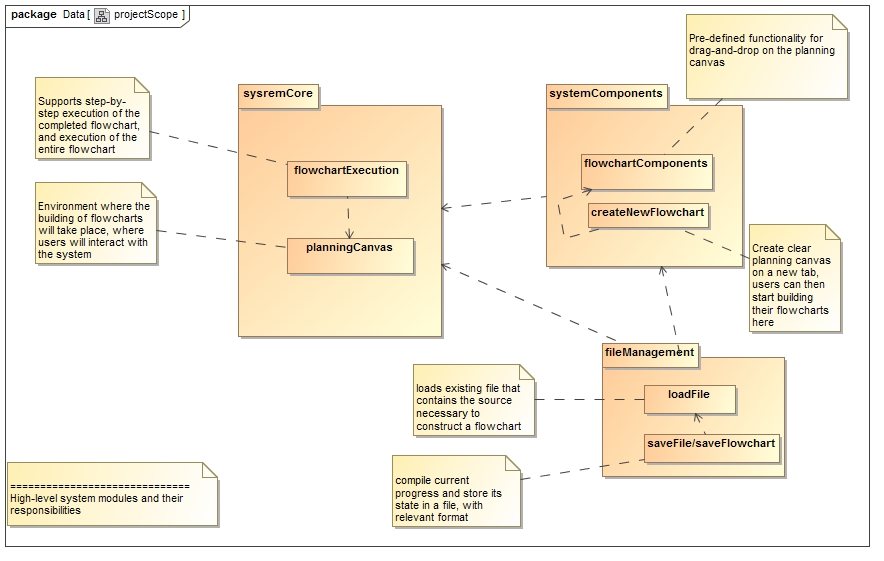
\includegraphics[width=500px]{projectScope.jpg}
\caption{High-level system modules and their responsibilities}
\end{figure}
% Include auxillary files here:  \input{file} 


\newpage	
\section{Use case prioritization}


\begin{table}[h!]   
    \label{tab:table1}
    \begin{tabular}{ccc}
      \toprule
      Critical & Important & Nice-To-Have\\
      \midrule	
      createFlowchartProject & addFlowchartComponent &  drag-and-drop components into bin\\
      deleteFlowchart & editFlowchartComponent & snap-to-grid development\\
       & deleteFlowchartComponent & predefined math functions\\
       & saveFlowchart & infinite-loop detection\\
       & loadFlowchart & logical-error detection\\
       & executeFlowchart & look-and-feel modification\\
      \bottomrule     
     \end{tabular}  
    \caption{Use case prioritization}
\end{table}


\newpage
\section{Use cases}

\subsection{createFlowchartProject}
Creates an environment to enable users to start building flowcharts.\newline\newline
\textbf{Pre Condition:} Planning canvas must be blank.\newline\newline
\textbf{Post Condition:} New canvas with Start and Return component created.\newline
\textbf{Post Condition:} Flowchart Planning and Simulation tools ready for use.\newline

\begin{figure}[H]
  \centering
\includegraphics[width=500px]{createNewFlowchartProject.eps}
\caption{createFlowchartProject Use Case Diagram}
\end{figure}

\begin{figure}[H]
  \centering
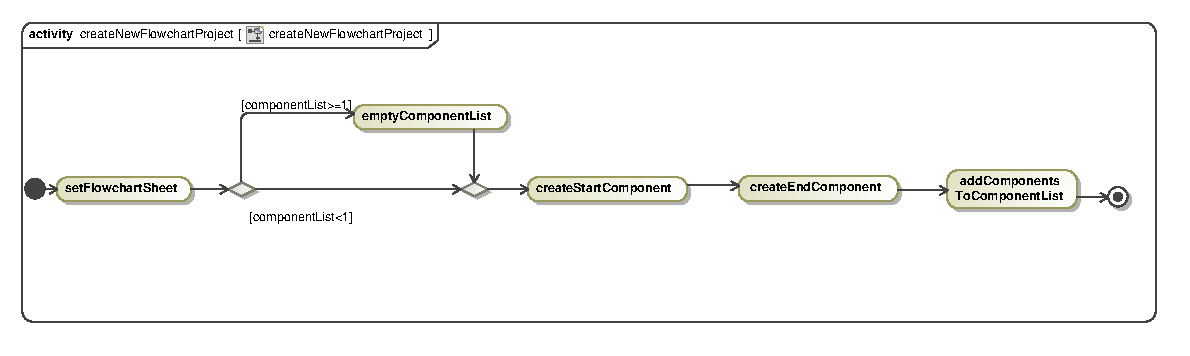
\includegraphics[width=500px]{createNewFlowchartProjectActivity.eps}
\caption{createFlowchartProject Activity Diagram}
\end{figure}

\newpage
\subsection{addFlowchartComponent}

Provides users with functionality to select the flowchart components they wish to place on the planning canvas.\newline\newline
\textbf{Pre Condition:} Canvas is available.\newline\newline
\textbf{Post Condition:} Component has been added to flowchart and appers on canvas with the necessary connections, if any.

\begin{figure}[H]
  \centering
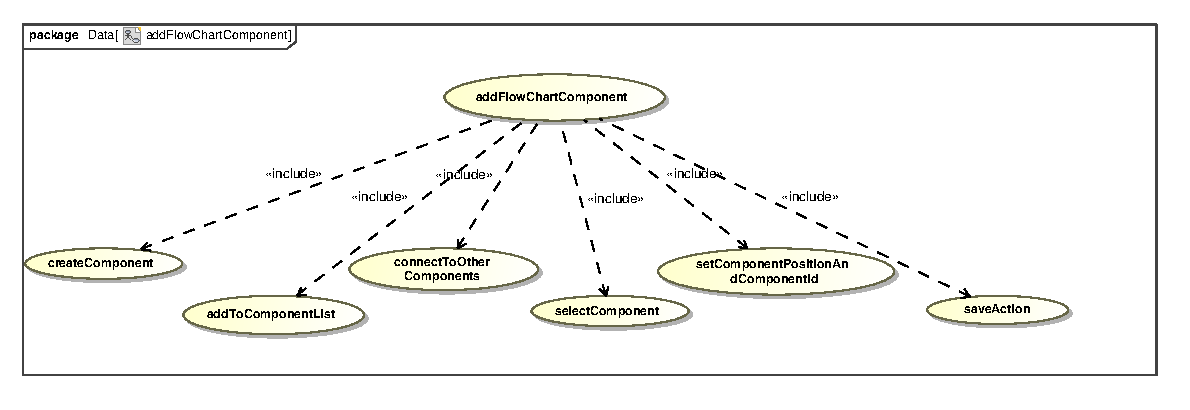
\includegraphics[width=500px]{addFlowChartComponent.eps}
\caption{addFlowchartComponent Use Case Diagram}
\end{figure}

\begin{figure}[H]
  \centering
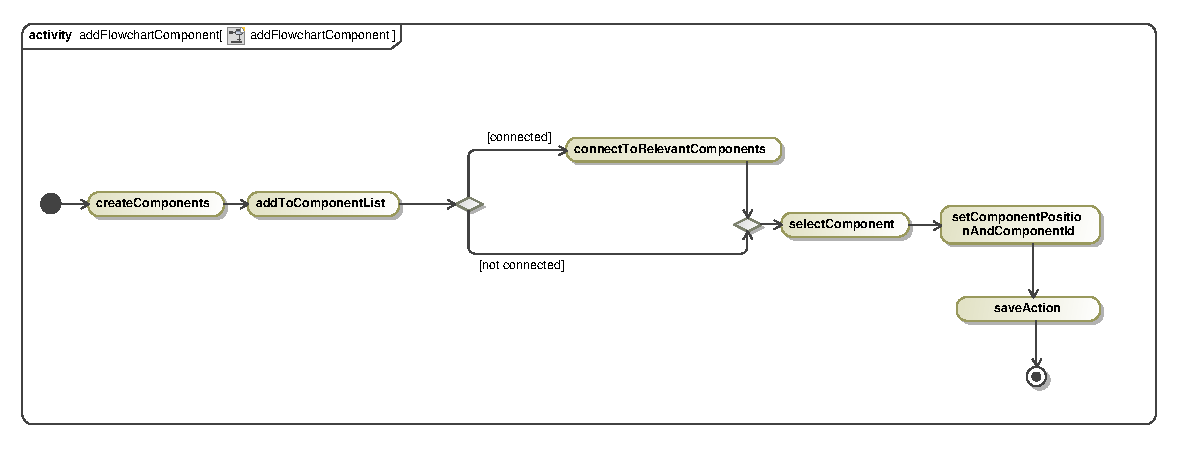
\includegraphics[width=500px]{addFlowchartComponentActivity.eps}
\caption{addFlowchartComponent Activity Diagram}
\end{figure}

\newpage
\subsection{editFlowchartComponent}

The editFlowchartComponent use case provides functionality for the user to edit each component of the flowchart on the canvas \newline\newline
\textbf{Pre Condition:} Canavas must exist.\newline
\textbf{Pre Condition:} Component must exist on active canvas.\newline\newline
\textbf{Post Condition:} Component has been edited.\newline
\textbf{Post Condition:} Edited component has been saved.

\begin{figure}[H]
  \centering
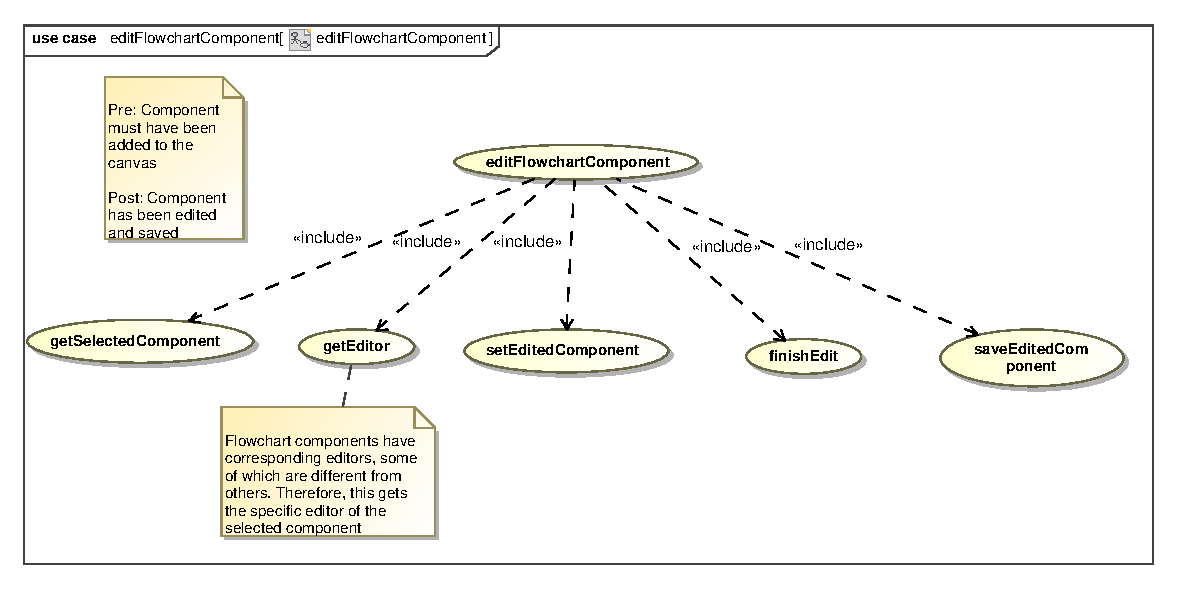
\includegraphics[width=500px]{editFlowchartComponent.eps}
\caption{editFlowchartComponent Use Case Diagram}
\end{figure}

\begin{figure}[H]
  \centering
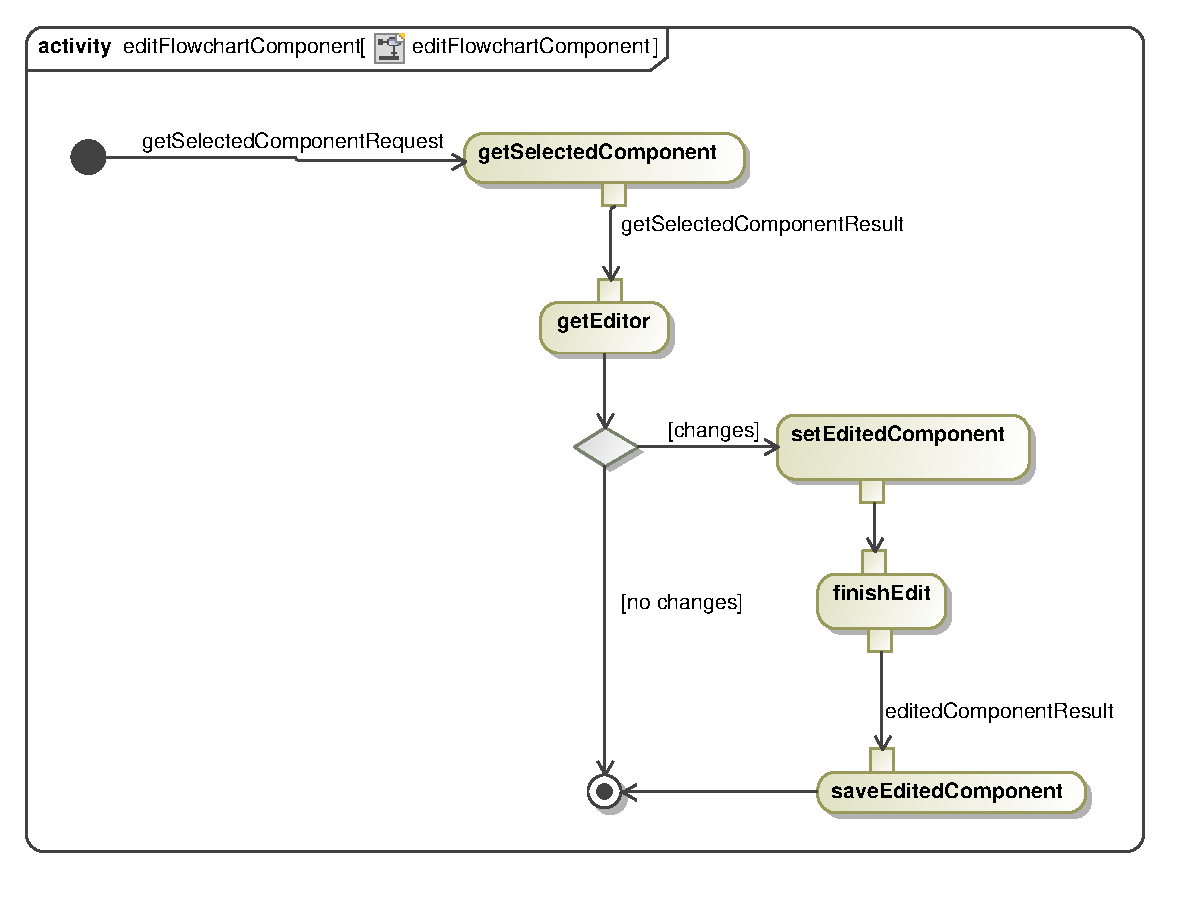
\includegraphics[width=300px]{editFlowchartComponentActivity.eps}
\caption{editFlowchartComponent Activity Diagram}
\end{figure}


\newpage
\subsection{deleteFlowchartComponent}
The deleteFlowchartComponent use case enables the functionality to delete individual components from the canvas.\newline\newline
\textbf{Pre Condition:} The canvas has to be available. \newline
\textbf{Pre Condition:} Component exists in the canvas space and is in the components list.\newline\newline
\textbf{Post Condition:} The canvas is clear of any components that were selected for removal.

\begin{figure}[H]
  \centering
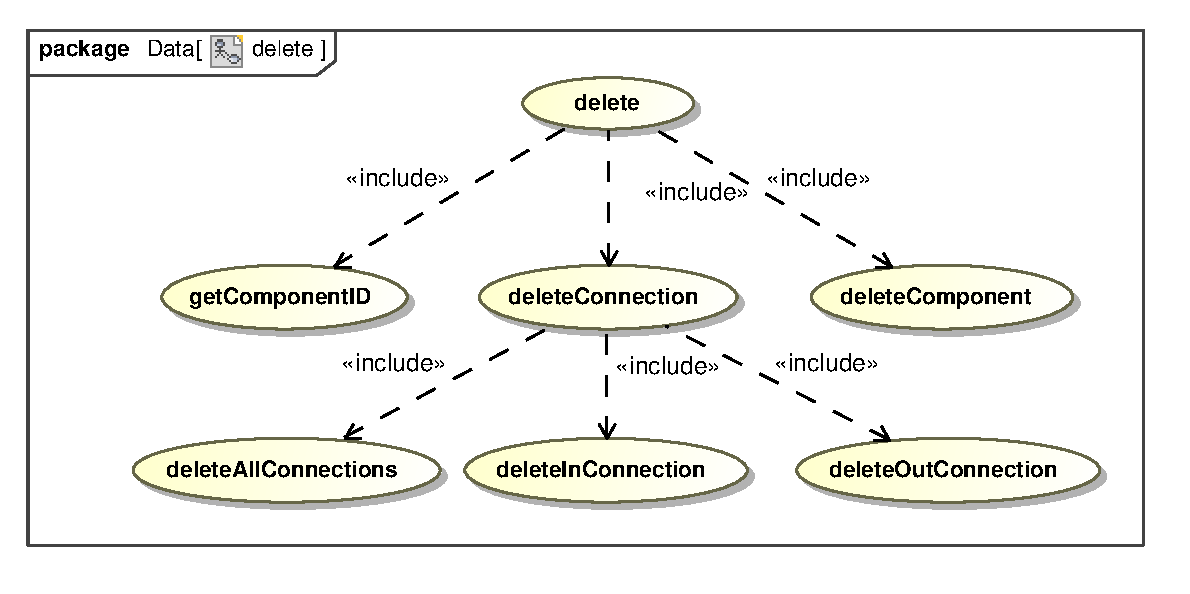
\includegraphics[width=500px]{delete.eps}
\caption{deleteFlowchartComponent Use Case Diagram}
\end{figure}

\begin{figure}[H]
  \centering
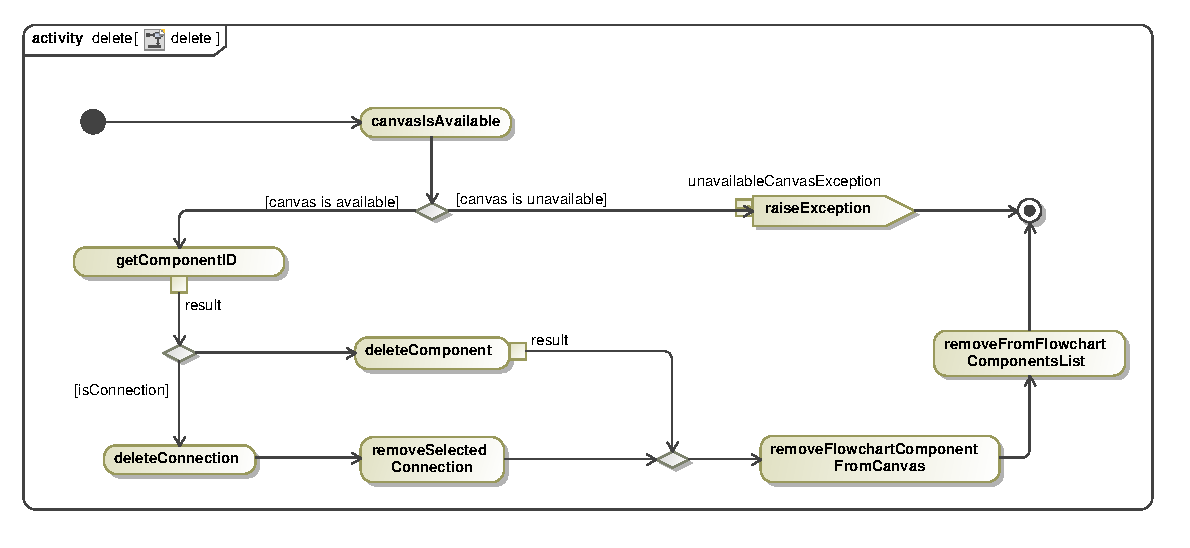
\includegraphics[width=500px]{deleteAct.eps}
\caption{deleteFlowchartComponent Activity Diagram}
\end{figure}

\newpage
\subsection{deleteFlowchart}
The deleteFlowchartProject use case serves the purpose of removing a flowchart project.\newline\newline
\textbf{Pre Condition:} Canvas exists.\newline
\textbf{Pre Condition:} Canvas is active.\newline
\textbf{Pre Condition:} The flowchart to be deleted must exist.\newline
\textbf{Pre Condition:} The flowchart to be deleted must be active.\newline\newline
\textbf{Post Condition:} The flowchart must be removed from the workspace and a new flowchart must then be created and made active on the workspace.

\begin{figure}[H]
  \centering
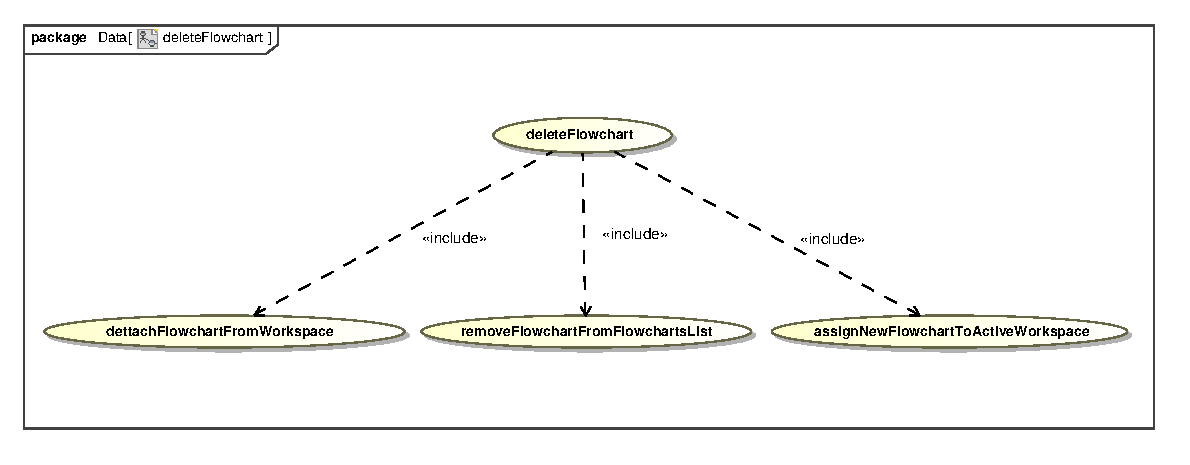
\includegraphics[width=500px]{deleteFlowchart.eps}
\caption{deleteFlowchart Use Case Diagram}
\end{figure}

\begin{figure}[H]
  \centering
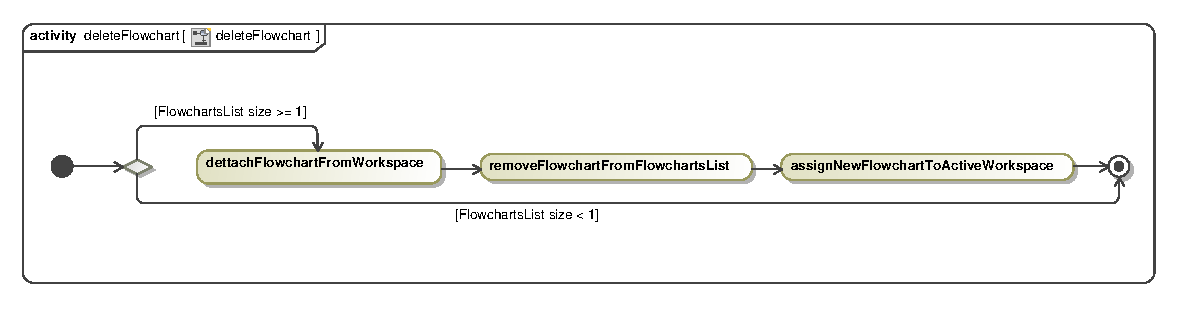
\includegraphics[width=500px]{deleteFlowchartActivity.eps}
\caption{deleteFlowchart Activity Diagram}
\end{figure}

\newpage
\subsection{saveFlowchart}
The saveFlowchart use case provides functionality for the user to save a flowchart.\newline\newline
\textbf{Pre Condition:} Canvas exists.\newline
\textbf{Pre Condition:} Canvas is active.\newline\newline
\textbf{Post Condition:} Flowchart has been saved to file.

\begin{figure}[H]
  \centering
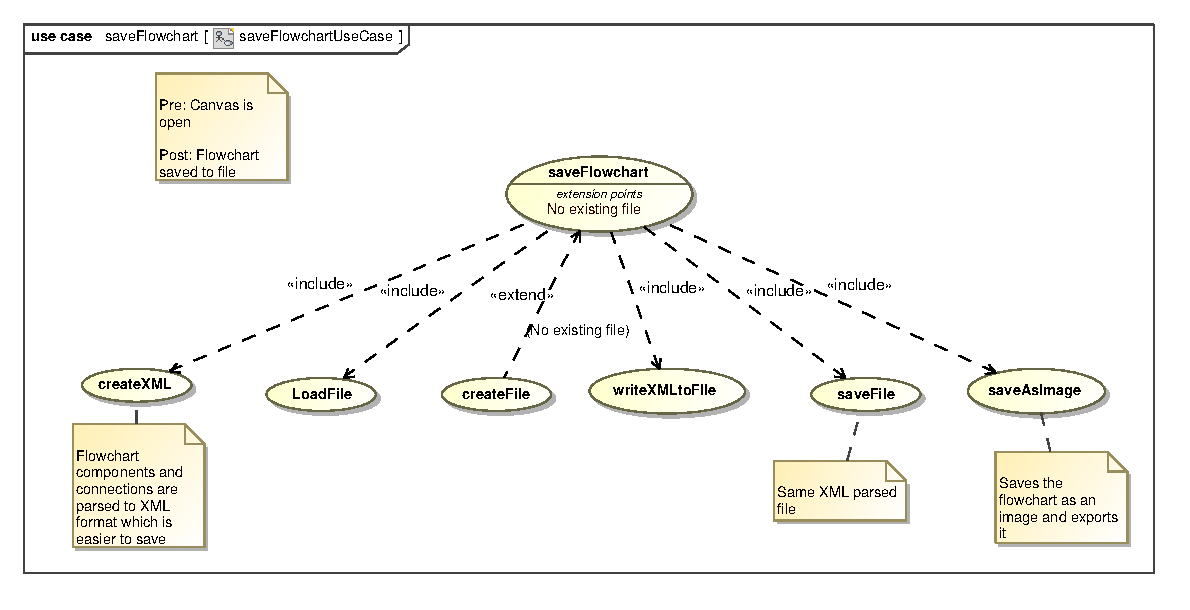
\includegraphics[width=500px]{saveFlowchartUseCase.eps}
\caption{saveFlowchart Use Case Diagram}
\end{figure}

\begin{figure}[H]
  \centering
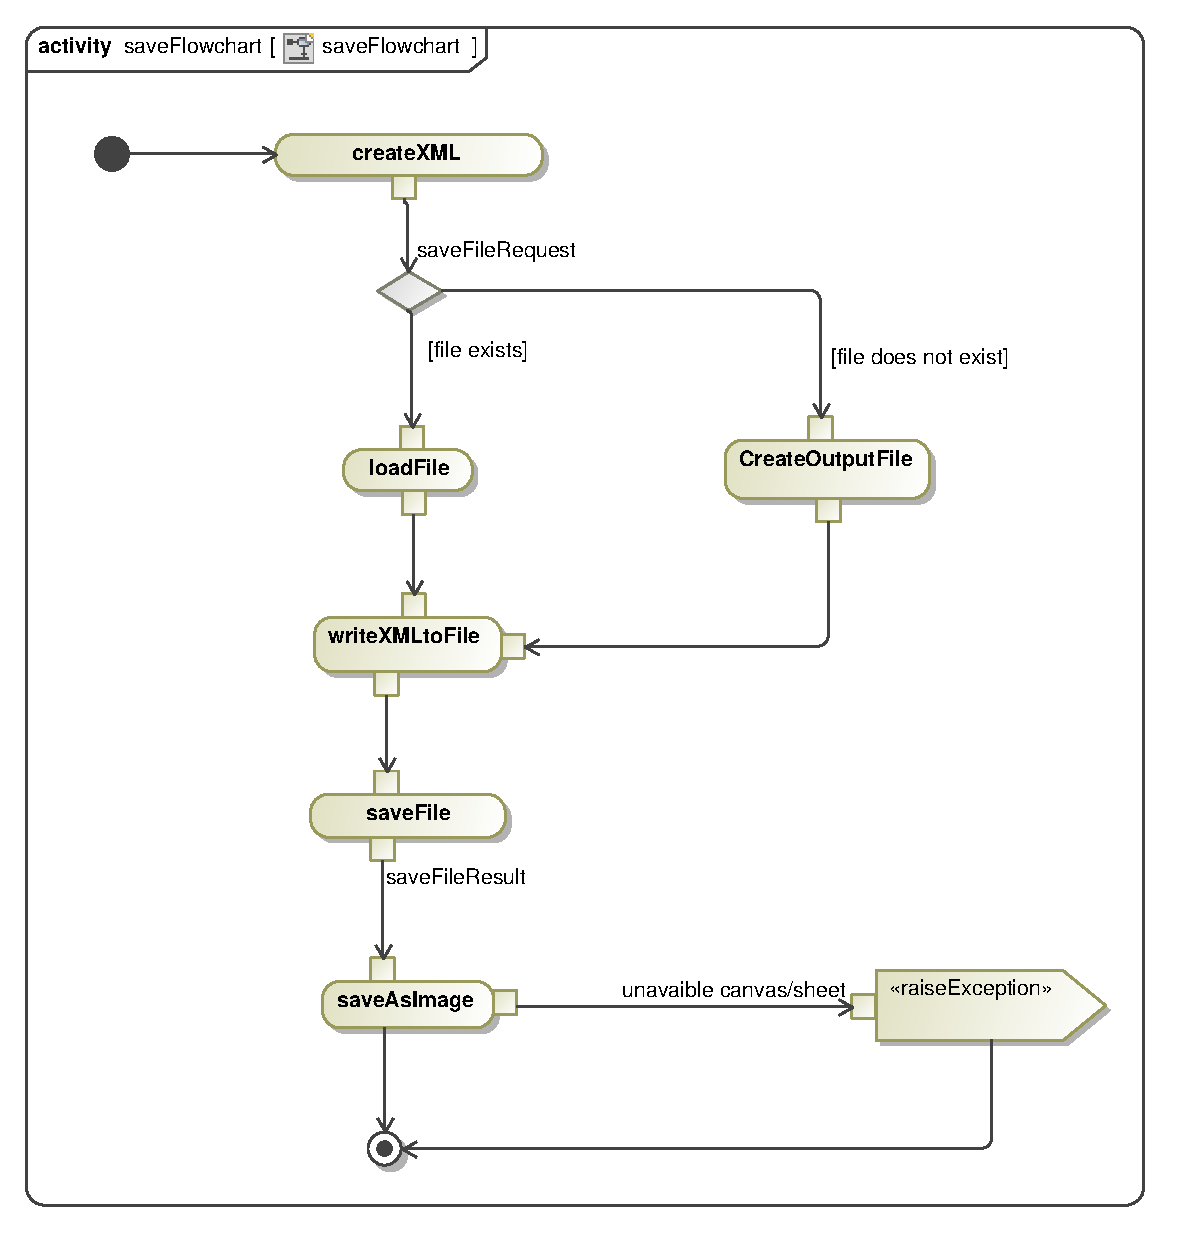
\includegraphics[height=250px, width=300px]{saveFlowchart.eps}
\caption{saveFlowchart Activity Diagram}
\end{figure}

\newpage
\subsection{loadFlowchart}
The loadFlowchart use case allows users load flowcharts from existing files. The file is editable and can be modified by the user.\newline\newline
\textbf{Pre Condition:} File with correct extension exists.\newline\newline
\textbf{Post Condition:} File contents have been converted and loaded on to the canvas.

\begin{figure}[H]
  \centering
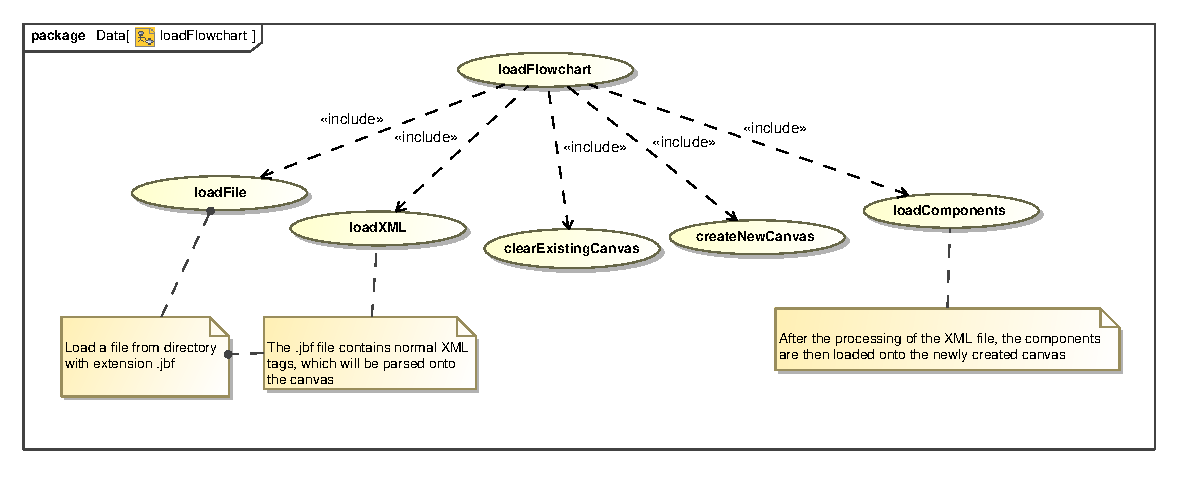
\includegraphics[width=500px]{loadFlowchart.eps}
\caption{loadFlowchart Use Case Diagram}
\end{figure}

\begin{figure}[H]
  \centering
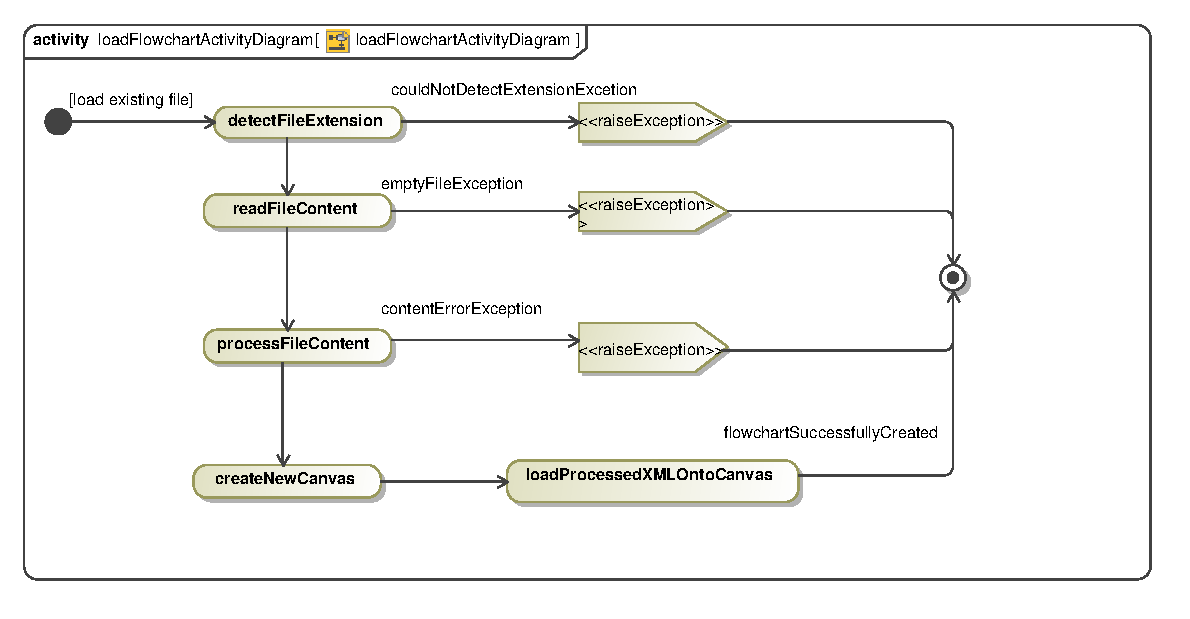
\includegraphics[width=500px]{loadFlowchartActivityDiagram.eps}
\caption{loadFlowchart Activity Diagram}
\end{figure}



\newpage
\subsection{executeFlowchart}
The executeFlowchart use case enables the functionality to execute the flowchart step-by-step or from start-to-end.\newline\newline
\textbf{Pre Condition:} Canvas has to be available.\newline\newline
\textbf{Post Condition:} Flowchart will return feedback of any errors, warnings or successful execution along with the results of any calculations.

\begin{figure}[H]
  \centering
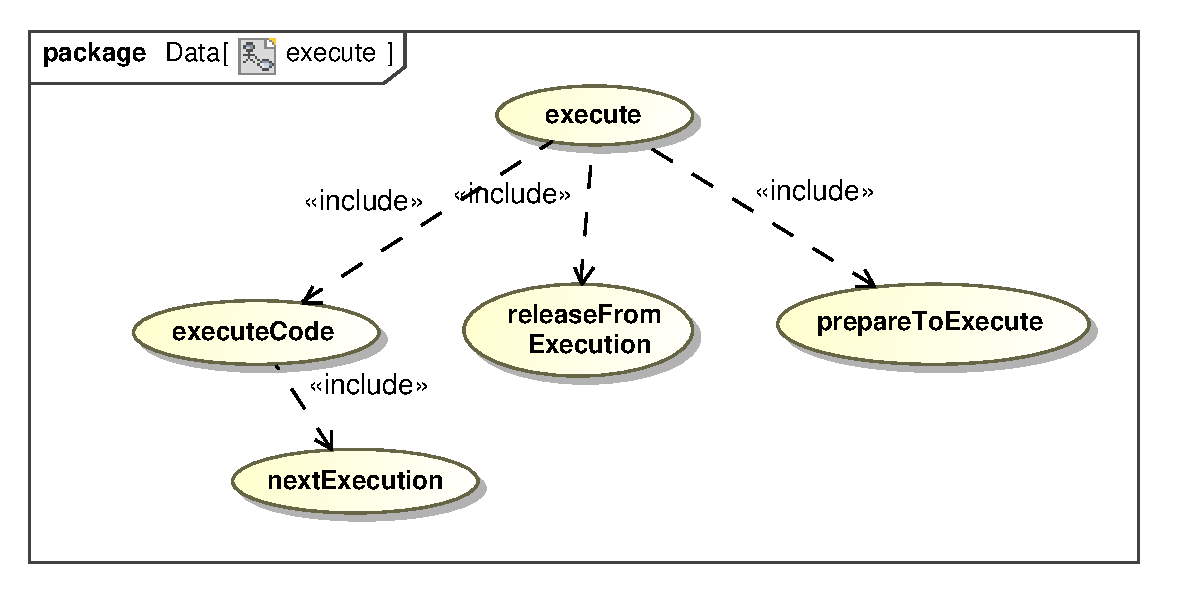
\includegraphics[width=500px]{execute.eps}
\caption{executeFlowchart Use Case Diagram}
\end{figure}

\begin{figure}[H]
  \centering
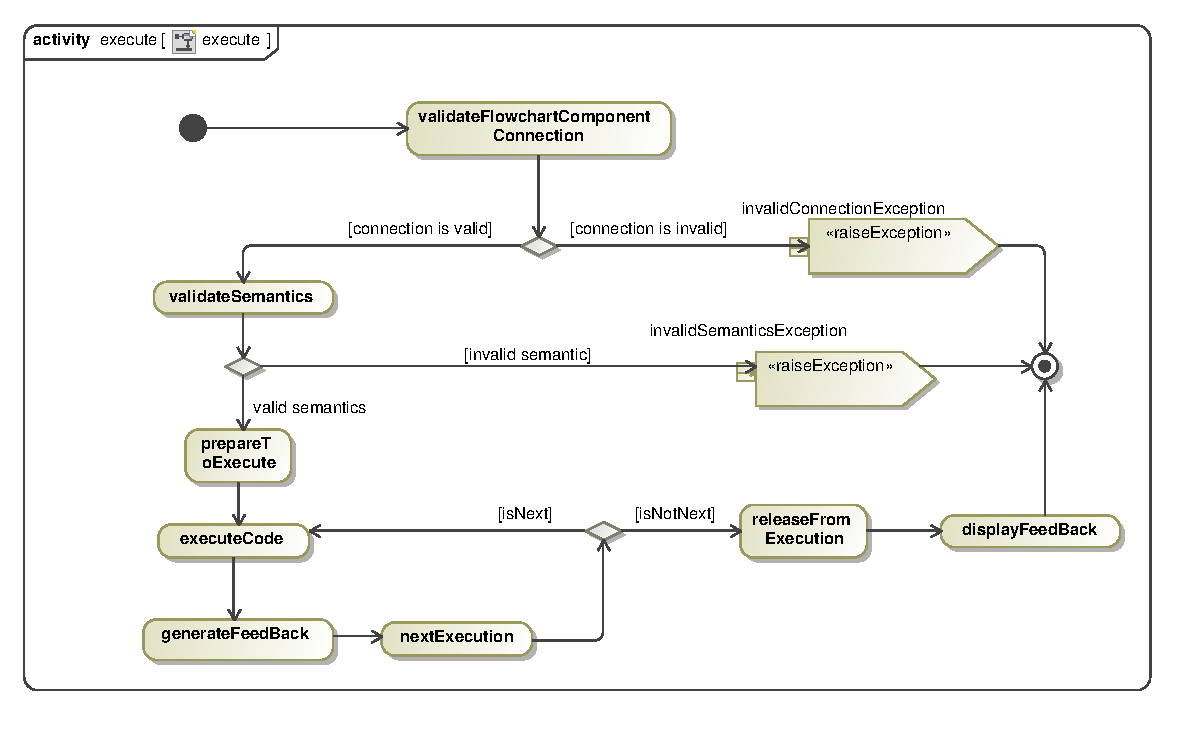
\includegraphics[width=385px]{executeAct.eps}
\caption{executeFlowchart Activity Diagram}
\end{figure}

\newpage
\section{The Domain Model - High-level}
\begin{figure}[H]
  \centering
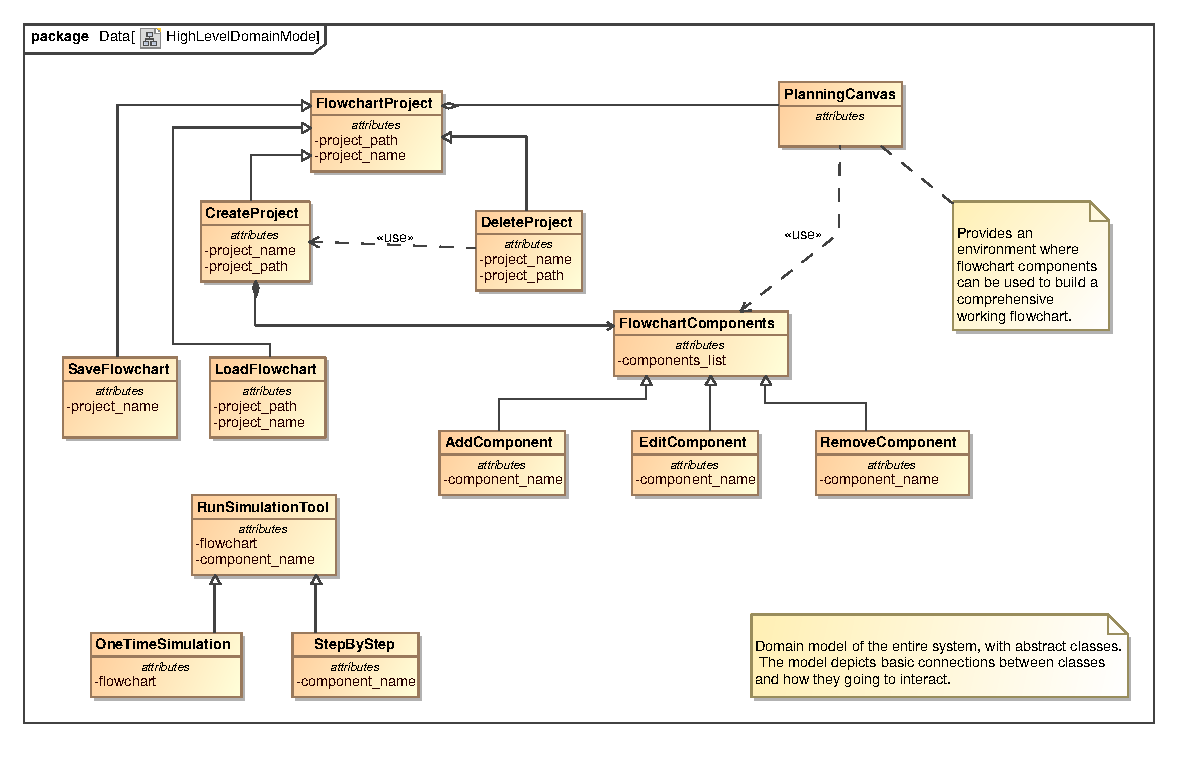
\includegraphics[width=500px]{HighLevelDomainModel.eps}
\caption{Domain Model Diagram}
\end{figure}

\end{document}
